\chapter{Numeryczny rozmyty regulator NPL}
	Rozmyty regulator numeryczny NPL różni się od regulatora SL sposobem liczenia aktualnej odpowiedzi swobodnej. Wszystkie elementy odpowiedzi swobodnej liczy się rekurencyjnie za pomocą wzorów od \ref{eq:npl1} do \ref{eq:npl3}, przy czym przyszłe odpowiedzi modelu $y_{k+i}^M$ liczy się rekurencyjnie z modelu rozmytego obiektu, zakładając przyszłe przyrosty sterowania równe 0.	Dalsza praca regulatora postępuje tak jak dla algorytmu SL, włącznie z obliczaniem zmiany sterowania za pomocą funkcji optymalizacji.
	
	12.3832
	

	\begin{equation}
		y_{k+i|k}^0=y_{k+i}^M+dk;
		\label{eq:npl1}
	\end{equation}
	\begin{equation}
		d_k = y_k-\sum_{i=1}^{D-1}\tilde{s}_i*\Delta u_{k-i}-\tilde{s}_D*u_{k-D}
		%-\sum_{i=1}^{Dz-1}\tilde{s}_i^z*\Delta z_{k-i}-\tilde{s}_{Dz}^z*z_{k-Dz}
		\label{eq:npl2}
	\end{equation}
	\begin{equation}
		y_{k}^M = \sum_{i=1}^{D-1}\tilde{s}_i*\Delta u_{k-i}+\tilde{s}_D*u_{k-D}
		%+\sum_{i=1}^{Dz-1}\tilde{s}_i^z*\Delta z_{k-i}+\tilde{s}_{Dz}^z*z_{k-Dz}
		\label{eq:npl3}
	\end{equation}
	
	Podczas pracy regulatora wartości horyzontów, lambda oraz kształt funkcji przynależności przyjęte zostały takie jak dla regulatora SL.
	
	\begin{figure}[h!]
		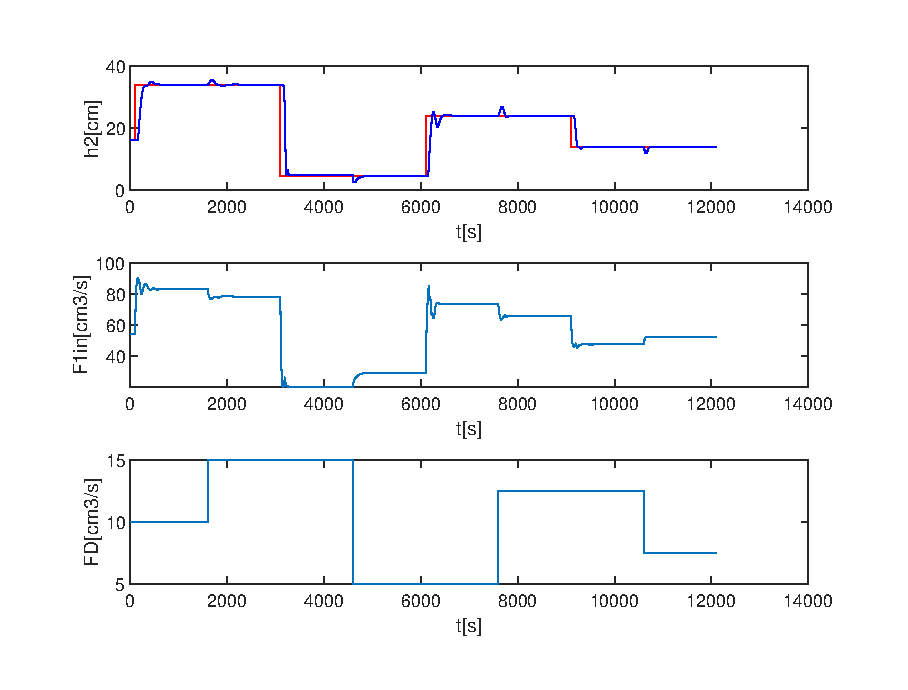
\includegraphics[width=0.9\linewidth]{plots/z3_fdmc_sl.eps}
		\caption{Przebieg regulacji dla numerycznego SL rozmytego}
		\label{rys:npl}
	\end{figure}

	Przebieg regulacji dla rozmytego regulatora numerycznego NPL przedstawiony został na wykresie \ref{rys:npl}. Porównując tenże wykres, z wykresem dla regulatora SL można stwierdzić, że przebiegi dla obydwu regulatorów są praktycznie identyczne i nie sposób jest znaleźć jakąkolwiek różnicę. Jeśli chodzi o porównanie przebiegu NPL oraz DMC, to sprowadza się one do jednej różnicy w działaniu opisanej już w poprzednim zadaniu. Błąd obliczony przy stosowaniu regulatora NPL wynosił 12.3832, tak więc nieco więcej niż przy regulowaniu SL, ale znacznie mniej niż dla DMC. Na podstawie powyższych spostrzeżeń nie można niestety stwierdzić czy użycie regulatora NPL jest lepsze czy gorsze od użycia regulatora SL. Wykresy są identyczne pod kątem wizualnym, a różnica w błędach niewielka. Jeśli chodzi o porównanie NPL oraz DMC, NPL wydaje się być nieco lepsze.